\documentclass{idrisMemo}
\usepackage{bookOfProof}
\usepackage{color}

\memoto{Idris}
\memosubject{Book of Proof}
\memodate{2024.03.23}
\status{\S 12.3 Pigeonhole Functions}

\begin{document}
\toc
\thispagestyle{styleTOC}
\pagebreak
\pagestyle{styleE}

\begin{prooflist}{1. Prove that if six integers are chosen at random, then at
    least two of them will have the same remainder when divided by 5 .}
    \item Let $A=\set{a_1, a_2, a_3, a_4, a_5, a_6}$.
    \item Let $B=\set{a\mid a \bmod 5, a\in\mathbb{N}}$.
    \item Let $f=A\rightarrow B$ be the function from $A$ to $B$.  Because
    $|A|=6>|B|=5$, $f$ cannot be injective and at least 2 elements from $a, b\in
    A, a\neq b$ result in $f(a)=f(b)$.
\end{prooflist}

\begin{prooflist}{2. Prove that if $a$ is a natural number, then there exist two
    unequal natural numbers $k$ and $\ell$ for which $a^k-a^{\ell}$ is divisible
by 10 .}
\item $f = (a^k - a^l) \mod 10$.
\item Let $A=\mathbb{N}\times\mathbb{N}$
\item Let $B=\set{a\mid a<10, a\in\mathbb{N}}$.
\item Let $f=A\rightarrow B$ be the function from $A$ to $B$.
\item Because the cardinality of $A$ is $\infty$ and the cardinality of $B$
    is 10, then $f$ cannot be injective. Therefore there exists values $k,
    l\in\mathbb{N}, k\neq l$ such that $(a^k-a^l)\mod 10\equiv 0$.
\end{prooflist}

\begin{prooflist}{3. Prove that if six natural numbers are chosen at random,
    then the sum or difference of two of them is divisible by 9 .}
\item Let $A=\set{a_1, a_2, a_3, a_4, a_5, a_6\mid a_i\in\mathbb{N}}$, $|A|=6$.
\item Let $B=\set{\set{0}, \set{1, 8},\set{2, 7},\set{3, 6},\set{4, 5}}$,
    $|B|=5$.
\item Let $f=A\rightarrow B$ be the function from $A$ to $B$. Because $|A|>|B|$,
$f$ is not injective. The function $f$ takes a natural number $a$ and then maps
the value $a\mod 9=b$ to the element of $B$ which contains $b$. For example
$f(10)=\set{1, 8}$, $f(40) = \set{4, 5}$, and $f(-18) = \set{0}$.

Because $f$ is not injective, 2 elements $a_i, a_j\in A$ will map to the same element
in $B$. We now show that $9\mid a_i+a_j \lor 9\mid a_i-a_j$.

\item First we consider the case when $f(a_i) = f(a_j) \neq \set{0}$. Suppose $a_i = 9\cdot n + r$, where $r$ is the remainder after dividing by
    9 and $n$ is some integer. Similarly $a_j=9\cdot m + s$, where $s$ is the
    remainder and $m$ is some integer. Because of the way $B$ is defined,
    $m+n=9$.
\begin{align*}
    a_i =& 9\cdot n + r\\
    a_j =& 9\cdot m + s\\
    a_i + a_j =& 9\cdot n + r + 9\cdot m + s\\
    a_i + a_j =& 9(n + r) + m + s \\
    a_i + a_j =& 9(n + r) + 9 \\
    a_i + a_j =& 9(n + r + 1)
\end{align*}
Therefore $9\mid a_i + a_j$.
\item Now we consider the case when $f(a_i) = f(a_j)= \set{0}$. Then $9\mid a_i
    \land 9\mid a_j$.
\begin{align*}
    a_i =& 9\cdot n\\
    a_j =& 9\cdot m\\
    a_i + a_j =& 9\cdot n + 9\cdot m\\
    a_i + a_j =& 9(n + r)
\end{align*}
Therefore $9\mid a_i + a_j$.
\item Thus we have proven the following statement
\quote{If six natural numbers are chosen at random,
    then the sum or difference of two of them is divisible by 9.}
\end{prooflist}

\begin{prooflist}{4. Consider a square whose side-length is one unit. Select any
    five points from inside this square. Prove that at least two of these points
are within $\frac{\sqrt{2}}{2}$ units of each other.}
\item Divide the unit square into 4 equal squares by bisecting each side of the
    original square. This results in 4 equal squares with sides of length
    $\dfrac{1}{2}$. The maximum distance between two points in the same smaller square is
    given by the diagonal of the smaller square. That diagonal $c$ has length
\begin{align*}
    a^2 + b^2 =& c^2\\
    \left(\frac{1}{2}\right)^2 + \left(\frac{1}{2}\right)^2 =& c^2\\
    \frac{1}{2} =& c^2\\
    \sqrt{\frac{1}{2}} =& c\\
    \frac{\sqrt{2}}{2} =& c
\end{align*}
By the pigeonhole principle, at least 2 points must be in the same square, and
the max distance of those points is $\frac{\sqrt{2}}{2}$.
\begin{figure}
   \centering
   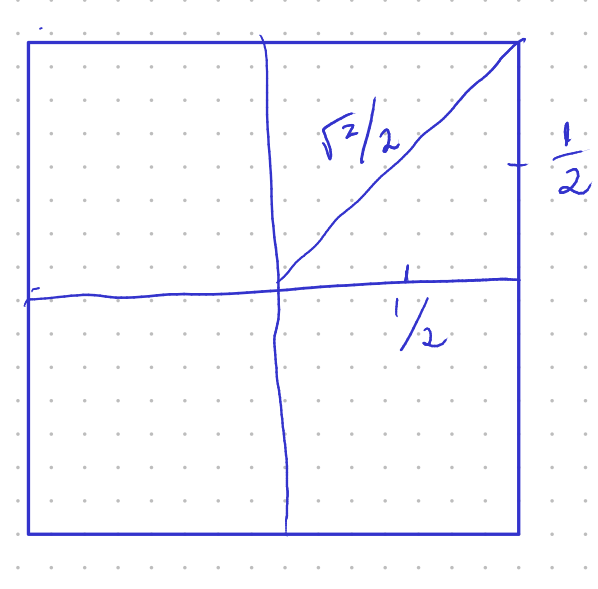
\includegraphics[width=0.5\textwidth]{images/12-03-04.png}
\end{figure}
\end{prooflist}

\begin{prooflist}{5. Prove that any set of seven distinct natural numbers
    contains a pair of numbers whose sum or difference is divisible by 10 .}
\item Let $A=\set{a_1, a_2, a_3, a_4, a_5, a_6, a_7\mid a_i\in\mathbb{N}}$, $|A|=7$.
\item Let $B=\set{\set{0}, \set{1, 9},\set{2, 8},\set{3, 7},\set{5}, \set{4, 6}}$,
    $|B|=6$.
\item Let $f=A\rightarrow B$ be the function from $A$ to $B$. Because $|A|>|B|$,
$f$ is not injective. The function $f$ takes a natural number $a$ and then maps
the value $a\mod 10=b$ to the element of $B$ which contains $b$. For example
$f(10)=\set{0}$, $f(41) = \set{1, 9}$, and $f(-18) = \set{2, 8}$.
Because $f$ is not injective, 2 elements $a_i, a_j\in A$ will map to the same element
in $B$. We now show that $10\mid a_i+a_j \lor 10\mid a_i-a_j$.
\item First we consider the case when $f(a_i) = f(a_j) \neq \set{0}$. Suppose
    $a_i = 10\cdot n + r$, where $r$ is the remainder after dividing by
    10 and $n$ is some integer. Similarly $a_j=10\cdot m + s$, where $s$ is the
    remainder and $m$ is some integer. Because of the way $B$ is defined,
    $m+n=10$.
\begin{align*}
    a_i =& 10\cdot n + r\\
    a_j =& 10\cdot m + s\\
    a_i + a_j =& 10\cdot n + r + 10\cdot m + s\\
    a_i + a_j =& 10(n + r) + m + s \\
    a_i + a_j =& 10(n + r) + 10 \\
    a_i + a_j =& 10(n + r + 1)
\end{align*}
Therefore $10\mid a_i + a_j$.
\item Now we consider the case when $f(a_i) = f(a_j)= \set{0}$. Then $10\mid a_i
    \land 10\mid a_j$.
\begin{align*}
    a_i =& 10\cdot n\\
    a_j =& 10\cdot m\\
    a_i + a_j =& 10\cdot n + 10\cdot m\\
    a_i + a_j =& 10(n + r)
\end{align*}
Therefore $10\mid a_i + a_j$.
\item Thus we have proven the following statement
\quote{Any set of seven distinct natural numbers
contains a pair of numbers whose sum or difference is divisible by 10.}
\end{prooflist}

\begin{prooflist}{6. Given a sphere $S$, a great circle of $S$ is the
    intersection of $S$ with a plane through its center. Every great circle
divides $S$ into two parts. A hemisphere is the union of the great circle and
one of these two parts. Prove that if five points are placed arbitrarily on $S$,
then there is a hemisphere that contains four of them.}
\item Select two of the five arbitrary points. With those two points and the
    center of the sphere, define a plane that bisects the sphere. The
    intersection of that plane and the sphere is a great circle $G$.
\item The remaining three points are placed in the two bisections defined by
    $G$. By the pigeonhole principle, one of those bisections $B_1$ has two of
    the remaining points.
\item A hemisphere is defined as the union of one of the bisections caused the
    by the great circle and the great circle itself. Therefore $H_1 = G \cup B_1$. $G$ has two points and
    $B_1$ has two points, therefore $H_1$ has four points.
\end{prooflist}

\begin{prooflist}{7. Prove or disprove: Any subset $X \subseteq\set{1,2,3, \ldots,
    2 n}$ with $|X|>n$ contains two (unequal) elements $a, b \in X$ for which
$a \mid b$ or $b \mid a$.}
\item Let $A=\set{1,2,3, \ldots, 2 n}$.
\item Let $X\subseteq A$ such that $|X|>n$.
\item Let $E(x)$ mean $x$ is even.
\item Let $O(x)$ mean $x$ is odd.
\item The set $A$ can be partitioned by parity---evens and odds.
\item Let $B=\set{x\in A \mid E(x)}$. Each $b\in B$ can be written as $b=2c$,
    for some integer $c\in A$.

\item Let $A_1=\set{1,2,3,4, 5, 6, 7, 8, 9, 10 }, n=5$.
\item Let $X_1=\set{1, 3, 5, 7, 9}, |X_1|=6$.

\item  Let us partition $A$ into two sets $B=\set{1\dots n}$ and
    $C=\set{n+1\dots 2n}$.
\item Each element of $C$ is either even or odd and can be written as either
    $2a$ or $2b+1$. For the even elements in $C$,
\item maybe partition into 4 sets?
\item Use the techniques from how to prove it.
\item To use the pigeonhole principle, devise a function that proves the point
    and is not injective
\item $f :: \mathbb{N} \rightarrow ? $
\item to linger upon ...
\end{prooflist}


\end{document}
